\documentclass{article}

\usepackage[T2A]{fontenc}
\usepackage[utf8]{inputenc}
\usepackage[russian]{babel}
\usepackage{mathtext}
\usepackage{textcomp}
\usepackage{graphicx}
\graphicspath{ {./images/} }
\usepackage{color}
\usepackage{xspace}
% \usepackage[document]{ragged2e}
\usepackage{multirow}
\usepackage{amsmath,amsfonts,amsthm,amssymb,amsbsy,amstext,amscd,amsxtra,multicol,mathtools}
\usepackage{indentfirst}
\usepackage{verbatim}
\usepackage{tikz}
\usepackage{forest}
\usepackage{soul} % зачеркивание

	
\usepackage[most]{tcolorbox}
\definecolor{block-gray}{gray}{0.90} % уровень прозрачности (1 - максимум)
\newtcolorbox{myquote}{colback=block-gray, grow to right by=0mm, grow to left by=0mm,
boxrule=0pt,boxsep=0pt,breakable} % настройки области с изменённым фоном

\usetikzlibrary{automata,positioning,graphs}
\usepackage[colorlinks,urlcolor=blue]{hyperref}

\usetikzlibrary{arrows.meta, shapes.geometric, calc}

\tikzstyle{startstop} = [
    ellipse,
    minimum width  = 3cm, 
    minimum height = 1 cm, 
    text centered, draw = black]

\tikzstyle{io} = [
    trapezium, 
    trapezium left angle  = 70,
    trapezium right angle = 110, 
    minimum width         = 3 cm, 
    minimum height        = 1 cm, 
    text centered, 
    draw=black]

\tikzstyle{process} = [
    rectangle, 
    minimum width  = 3 cm, 
    minimum height = 1 cm,
    text centered, 
    draw=black]

\tikzstyle{decision} = [
    diamond, 
    minimum width  = 3 cm, 
    minimum height = 1 cm,
    text centered, 
    draw=black]

\tikzstyle{arrow} = [
    thick,
    ->,
    >=stealth]

\setlength{\parindent}{0.8cm}
\setlength{\parskip}{0cm}

\def\eps{\varepsilon}
\usepackage[left =2cm, right=2cm, top=2cm, bottom=2cm, bindingoffset=0cm]{geometry}

\begin{document}
\author{Лабунец Л. В.}
\title{Нейронные сети. Лекции.}
\maketitle

% \setcounter{section}{4}
\section*{Лекция}
\addtocounter{section}{1}

\subsection{Математическая модель многослойного перцептрона}

Рассмотрим на примере 3-слойной архитектуры (в количество слоёв входят только слои, реализующие нелинейное отображение).
Рассмотрим сигналы, поступающие на вход нейронов, но для избежания путаницы, будем визуализировать связи только для первых нейронов соответствующих слоёв.
Рассмотрим эти связи и соотв. им параметры.

\begin{figure}[htbp]
    \centering
    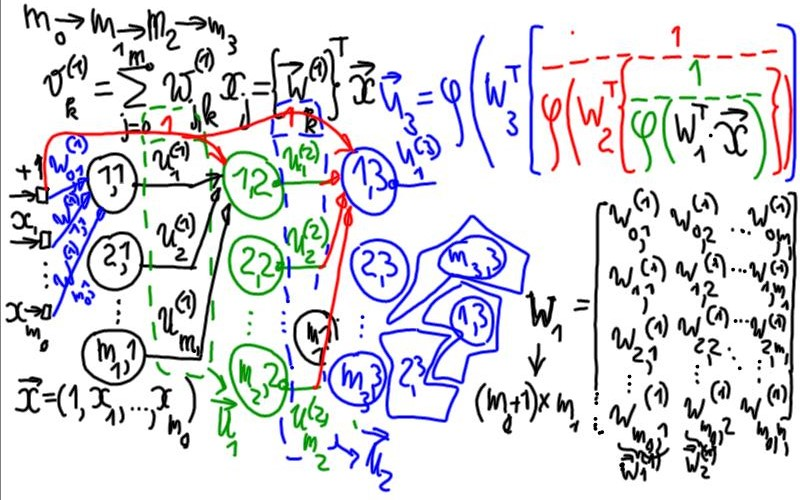
\includegraphics[width=\textwidth]{hyperflat_3_1.jpeg}
    \caption{Структура многослойного перцептрона}
    % \label{<label>}
\end{figure}

3-слойный перцептрон содержит 0-й слой - слой источников (черные квадратики). 
Имеется $m_{0}$ входов, на которые поступают признаки $\vec{x} = (1, x_0, ..., x_{m_{0}})$, 3 скрытых слоя.

Примем следующие правила индексации скрытых нейронов и нейронов выходного слоя:
первый эл-т индекса - номер нейрона, второй - номер слоя: $m_{i,j}$  - $i$-й нейрон $j$-го скрытого слоя.

Выпишем веса нейронов $i$-го слоя в виде матрицы $W_i$, столбец которой $\vec{w}_i^{(k)}$ является вектором весов $i$-го нейрона $k$-го слоя.
Количество строк матрицы - количество входов слоя + 1 (на вход поступает расширенный вектор), количество столбцов - количество нейронов слоя.
Элемент матрицы $w_{i,j}^{(k)}$ - вес $i$-го входа $j$-го нейрона $k$-го слоя.
У первого скрытого слоя имеется $m_0$ входов (слой источников) и он содержит $m_1$ нейронов.

\begin{equation}
    W_1 = 
    \begin{pmatrix}
        w_{0,1}^{(1)} & w_{0,2}^{(1)} & \dots & w_{0,{m_1}}^{(1)} \\
        w_{1,1}^{(1)} & w_{1,2}^{(1)} & \dots & w_{1,{m_1}}^{(1)} \\
        w_{2,1}^{(1)} & w_{2,2}^{(1)} & \dots & w_{2,{m_1}}^{(1)} \\
        \vdots        & \vdots        & \ddots & \vdots           \\
        w_{{m_0},1}^{(1)} & w_{{m_0},2}^{(1)} & \dots & w_{{m_0},{m_1}}^{(1)} \\
    \end{pmatrix}
\end{equation}

Рассмотрим первый слой.
На вход каждого нейрона слоя поступает сигнал смещения $+1$, взвешиваемый \textit{биасом} $w_{0,i}^{(1)}$. 
Также на вход этого нейрона поступают входные признаки $x_i$, взвешиваемые \textit{синаптическими весами} $w_{1,j}^{(1)}$ до $w_{{m_0},j}^{(1)}$ - веса $i$-го признака $j$-го нейрона в первом слое.   
Для экономии места введём вектор синаптических весов конкретного нейрона:

\begin{equation}
    \vec{w}_j^{(k)} = 
    \begin{pmatrix}
        w_{0,j}^{(k)} & w_{1,j}^{(k)} & \dots & w_{{m_0},j}^{(k)}
    \end{pmatrix}
    ^T
\end{equation}


Индекс в скобках - номер слоя, нижний индекс - номер нейрона. Т.е., $\vec{w}_1^{(1)}$ - вектор синаптических весов 1-го нейрона 1-го слоя.

На выходе $i$-го нейрона $k$-го слоя формируется сигнал $u_i^{(k)}$. 
Выпишем формулу для вычисления сигнала на выходе 1-го нейрона 1-го слоя $u_1^{(1)}$. Опять, в скобках - номер слоя, индекс - номер нейрона.
Для этого необходимо посчитать сигнал на выходе сумматора $k$-го нейрона (\textit{индуцированного локального поля}):

\begin{myquote}
    \textit{Не очень удачно были выбраны индексы, но оставил, как на презентации}
\end{myquote}

\begin{equation}
    {v}_k^{(1)} = \sum_{j=0}^{m_0} w_{j,k}^{(1)} \cdot x_j = [\vec{w}_{k}^{(1)}]^T \cdot \vec{x}
\end{equation}


\begin{equation*}
    {v}_2^{(1)} = [\vec{w}_{2}^{(1)}]^T \cdot \vec{x}
\end{equation*}

где $j$ - номер нейрона, $k$ - номер слоя, $w_{j,k}^{(1)}$ - компоненты ..., $\vec{x}$ - расширенный вектор.

Из приведённых выражений можем получить общее: $W_k^T \cdot \vec{x}$ - совокупность элементов на выходе сумматоров всех нейронов $k$-го слоя.

Полученные на выходе сумматора значения подвергаются нелинейному преобразованию с помощью функции активации $\varphi(W_k^T \cdot \vec{x})$. Получаем совокупность сигналов на выходе функций активации нейронов. 
Для первого слоя: $\varphi(W_1^T \cdot \vec{x})$, для второго: $\varphi(W_2^T \cdot \vec{x})$ и т.д.

Для получения из матрицы $W_1$ матрицы $W_2$ рисуем таблицу:

\begin{center}
    Количество входов и выходов скрытых слоёв (без учёта "расширенности" векторов):

    \begin{tabular}{c | c |  c | c |}
        & 1 слой & 2 слой & 3 слой \\
        \hline
        Количество входов  & $m_0$ & $m_1$ & $m_2$ \\
        \hline
        Количество выходов & $m_1$ & $m_2$ & $m_3$ \\
        \hline
    \end{tabular}
\end{center}

Выпишем матрицу $W_2$;
\begin{equation}
    W_1 = 
    \begin{pmatrix}
        w_{0,1}^{(2)} & w_{0,2}^{(2)} & \dots & w_{0,{m_2}}^{(2)} \\
        w_{1,1}^{(2)} & w_{1,2}^{(2)} & \dots & w_{1,{m_2}}^{(2)} \\
        w_{2,1}^{(2)} & w_{2,2}^{(2)} & \dots & w_{2,{m_2}}^{(2)} \\
        \vdots        & \vdots        & \ddots & \vdots           \\
        w_{{m_1},1}^{(2)} & w_{{m_1},2}^{(2)} & \dots & w_{{m_1},{m_2}}^{(2)} \\
    \end{pmatrix}
\end{equation}

И получим выходы сумматоров нейронов второго слоя:

\begin{myquote}
    Починить расширенные вектора!
\end{myquote}

\begin{equation}
    \vec{u}_2 = W_2^T \cdot [\dfrac{1}{\varphi(W_1^T \cdot \vec{x})}]
\end{equation}


В формуле 1 в якобы числителе - добавленный первый элемент, чтобы получить расширенный вектор-столбец.

\begin{equation}
    \vec{u}_3 = \varphi(W_3^T[\dfrac{1}{\varphi(W_2^T \cdot [\dfrac{1}{\varphi(W_1^T \cdot \vec{x})}])}])
\end{equation}

Для 4-го слоя получим:

\begin{myquote}
    \textit{Выписать матрицу с рисунка для 4 слоя, поправить формулу и выписать её}
\end{myquote}

Увеличение слоёв нецелесообразно из-за рекурсивной структуры модели многослойного перцептрона (последовательность вложенных блоков),
что приводит к уменьшению скорости вычисления, увеличению занимаемой памяти и накопления ошибок.
Также по мере увеличения параметров модели, возникает \textit{эффект переобучения}, а по мере увеличения количества слоёв, количество параметров увеличивается экспоненциально.

Возможно применение альтернативных архитектур - например, сети радиальных базисных функций.
Также необходимо применение методов регуляризации, например, метод \textit{хирургии мозга} - исключения из каждого слоя неинформативных нейронов или целых слоёв.
Существуют методы обучения, подразумевающие цикличность. Более детально см. "Нейронные сети. Полный курс" Саймона Хайкина (?).

Также существует теорема, доказанная Колмогоровым, утв., что многомерная скалярная функция может воспроизводить любую закономерность сколь угодно большой сложности. Теорема об универсальной аппроксимации многослойным перцептроном, утв., что архитектура многослойного перцептрона \textit{теоретически} позволяет с любой заданной точностью синтезировать
многомерную по количеству входов векторную функцию, что позволяет строить модели нелинейных дискриминантных границ в пространстве признаков и, соотв., определять принадлежность
данных кластерам. 

\subsection{Системный подход к синтезу алгоритмов обучения многослойного перцептрона}


\begin{myquote}
    \textit{Рисунок hyperrflat 5 1}
\end{myquote}

Системный подход к синтезу алгоритмов обучения многослойного перцептрона
\begin{enumerate}
    \item Выбор цели обучения;
    \item Оценка градиента средних потерь целевой функции по параметрам нейронной сети;
    \item Использование алгоритмом поиска оптимальных параметров.
\end{enumerate}

Предполагается наличие функционала качества работы системы, оптимальное значение которого и ищется.

Будем рассматривать 3 объекта анализа
\begin{enumerate}
    \item Пространство входных воздействий $\vec{x}$ - сигналы, поступающие на вход системы (обучающие и контрольные примеры), и соответствующее пространство входных воздействий, в котором существует область $D$ все возможных входных воздействий;
    \item Вектор параметров системы $\vec{C}$ и пространство, ему соответствующее, в которому существуют эквипотенциальные гиперповерхности, все точки которых соотв. определенным значениям функционала качества. Необходимо найти область мимальных/максимальных значений этого функционала качества;
    \item Функция стоимости (потерь, приобретений) $Q(\vec{x}, \vec{c})$, определяющая потери/приобретения, которые можно измерить, если на вход системы поступает воздействие $\vec{x}$, а система находится в в состоянии $\vec{C}$.
\end{enumerate}

Набор этих 3 объектов позволяет математически строго сформулировать выбор цели обучения в виде функционала средних потерь (среднего риска).
Сделать это несложно, необходимо протестировать область $D$ всех входных воздействий: зафиксировать $\vec{x}$ и выбрать параметры системы $\vec{C}$. 
Для каждого зафиксированного выбора параметров системы необходимо вычислить потери по выбранной для кажого вхожного воздействия и просуммировать их:

\begin{equation}
    J(\vec{C}) = \int_{D} Q(\vec{x}, \vec{C}) p(\vec{x}) d\vec{x}
\end{equation}

Полученное $J(\vec{C})$ - средний риск (средние потери), $p(\vec{x})$ - весовая функция, сглаживающая аномальные значения (плотность распределения вероятностей входных воздействий).

На практике возможны 2 ситуации:
\begin{enumerate}
    \item Нетипичный случай полной априорной определённости - полное знание входных воздействий (весовой функции $p(\vec{x})$, Типа распределения и тд.);
    \item Типичный случай - функция задана набором обучающий примеров
\end{enumerate}

Во втором случае необходимо выполнить предварительную выборочную оценку весовой функции $p(\vec{x})$ по набору обучающих примеров.
\begin{myquote}
    \textit{Рисунок hyperflat 4 1}
\end{myquote}

Однако, будем считать весовую функцию $p(\vec{x})$ известной, тогда возможно посчитать функционал ошибок $J(\vec{C})$.

\paragraph{Алгоритм обучения нейронной сети (метод градиентного поиска):}
\begin{enumerate}
    \item Выбрать начальное приближение параметров нейронной сети $\vec{C}[0]$, $0$ - номер итерации, и оценить потери;
    \item Выбрать оптимальное направление поиска (вектор антиградиента $-\nabla\vec{C}$, указывающий направление, в котором потери убывают с максимальной скоростью);
    \item Выбрать шаг поиска (используется процедура стохастической аппроксимации Роббенса-Монро, в соответствии с которой с каждой итерацией длина шага уменьшается обратно пропорционально номеру итерации);
    \item[] В полученной точке выполняется подтверждение сходимости (сравнение итераций), вычисление нового напраление и шага.
\end{enumerate}

Процедура описывается следуюшим выражением:

\begin{equation}
    \vec{C}[i] = \vec{C}[i-1] - \Gamma[i] \nabla\vec{C} \{ J(\vec{C}[i-1]) \}
\end{equation}

Цель обучения: 

\begin{equation}
    \vec{C}_{opt} = \arg \min_{\vec{C}} \{ J(\vec{C}) \}
\end{equation}

Существуют также методы, не требующие вычилсения частной производной, - метод деформируемого многоранника Нелдера-Мида (симплекс-поиск).

\begin{myquote}
    \textit{Прикладное нелинейное программирование, Химмельблау}
\end{myquote}

Обучение сводится к решению задачи оптимизации. Существуют ограничения на значения параметров системы в виде равенств или неравенств.

Результаты выполнения алгоритма зависят от выбора начального приближения, что приводит к необходимости выбора нескольких начальных приближений для обнаружения всех локальных минимумов.
Существенное преимущество в этом случае обеспечивают генетические алгоритмы.

\subsection{Алгоритм обучения нейронной сети для случая набора обучающих примеров}






\end{document}